\chapter{Strategy}
\begin{figure}[!ht]
\begin{center}
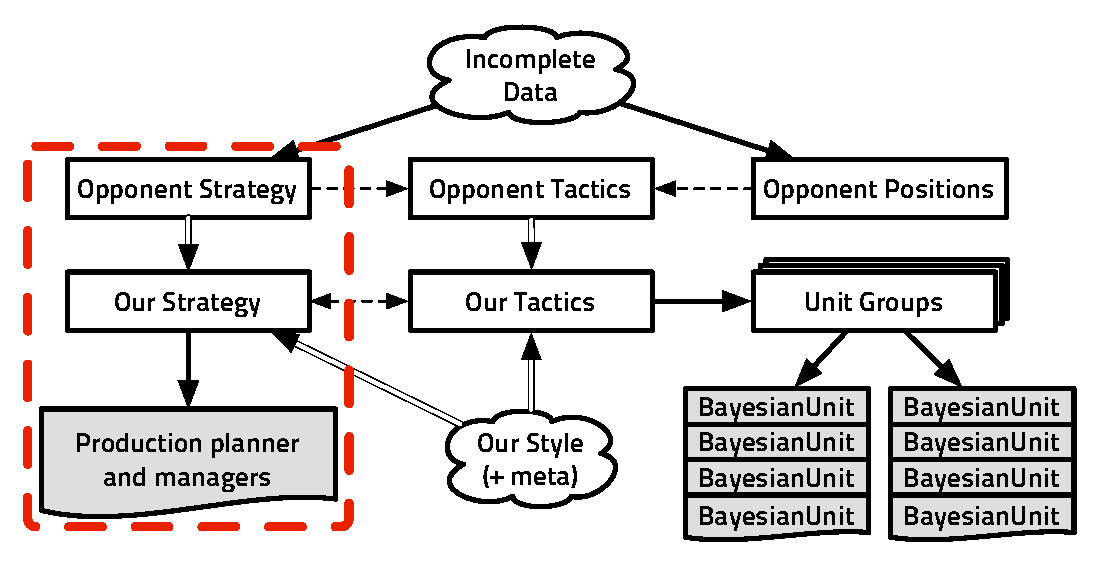
\includegraphics[width=13cm]{images/starcraft_bbq_concept_STRATEGY.pdf}
\end{center}
\label{fig:conceptSTRATEGY}
\caption{Information-centric view of the architecture of the bot, the part concerning this chapter is in the dotted rectangle}
\end{figure}
\begin{itemize}
\item Problem: take the winning strategy in the absolute
\item Complexity: without going meta, prediction is an ``inference under uncertainty'' problem, adaptation w.r.t. what we know is a planning under constraints problem. Going meta $\Rightarrow$ \texttt{(O.O)}
\item State of the art: Data mining, plan recognition, CBR... \citep{weberStrat}, \citep{Weber2010qf} and even meta \citep{metalevelbehavioradaptrts}.
\item Our take: \citep{SYNNAEVE:OpeningPred}, \citep{SYNNAEVE:StratPred}
\item Results: better resistance to noise, which is fundamental in real setup RTS gameplay (fog of war). Full Bayesian model down to adaptation actions some day?
\item Conclusion and perspectives: a way to encode and use gameplay/structural knowledge 
\end{itemize}


